\documentclass{standalone}
\usepackage{graphicx}
\usepackage[latin1]{inputenc}
\usepackage{tikz}
\usetikzlibrary{shapes, arrows}
%\tikzstyle{startstop} = [rectangle, rounded corners, minimum width=3cm, minimum height=1cm,text centered, draw=black, fill=red!30]
%\tikzstyle{io} = [trapezium, trapezium left angle=70, trapezium right angle=110, minimum width=3cm, minimum height=1cm, text centered, draw=black, fill=blue!30]
%\tikzstyle{process} = [rectangle, minimum width=3cm, minimum height=1cm, text centered, draw=black, fill=orange!30]
%\tikzstyle{decision} = [diamond, minimum width=3cm, minimum height=1cm, text centered, draw=black, fill=green!30]

\tikzstyle{startstop} = [rectangle, rounded corners, text centered, draw=black, fill=red!30]
\tikzstyle{io} = [trapezium, trapezium left angle=70, trapezium right angle=110,  text centered, draw=black, fill=blue!30]
\tikzstyle{process} = [rectangle, text centered, draw=black, fill=orange!30]
\tikzstyle{decision} = [diamond,  text centered, draw=black, fill=green!30]
\tikzstyle{arrow} = [thick,->,>=stealth]

\tikzset{->, 
>=stealth, node distance=3cm}
\begin{document}
        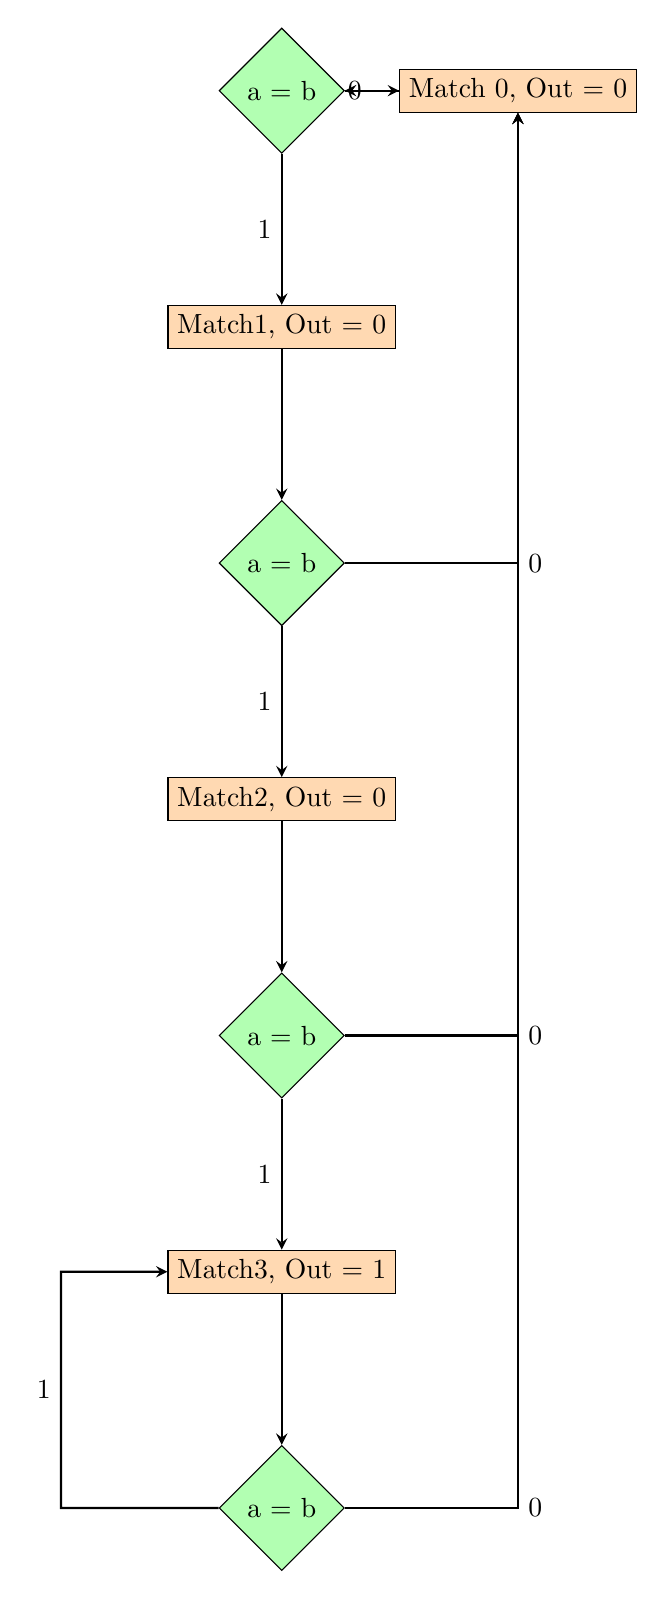
\begin{tikzpicture}
            
            \node (match0) [process]  {Match 0,  Out = 0 };
            \node (check1) [decision,left of=match0] {a = b };
            \node (match1) [process,below of=check1] {Match1, Out = 0 };
            \node (check2) [decision, below of=match1] {a = b };
            \node (match2) [process,below of =check2] { Match2, Out = 0 };
            \node (check3) [decision,below of =match2] {a = b };
            \node (match3) [process,below of =check3] { Match3, Out = 1 };
            \node (check4) [decision,below of =match3] {a = b };

            \draw [arrow] (match0) --  (check1);
            \draw [arrow] (match1) --  (check2);
            \draw [arrow] (match2) --  (check3);
            \draw [arrow] (match3) --  (check4);
            \draw [arrow] (check1) -- node[anchor=east] {0} (match0);
            \draw [arrow] (check2) -| node[anchor=west] {0} (match0);
            \draw [arrow] (check3) -| node[anchor=west] {0} (match0);
            \draw [arrow] (check4) -| node[anchor=west] {0} (match0);
            \draw [arrow] (check1) -- node[anchor=east] {1} (match1);
            \draw [arrow] (check2) -- node[anchor=east] {1} (match2);
            \draw [arrow] (check3) -- node[anchor=east] {1} (match3);
            \draw [arrow] (check4.west) -- ++(-2,0) -- node[anchor=east] {1} ++(0,3) -- (match3.west);

        \end{tikzpicture}
\end{document}
